\section{Tables}

\begin{table}[ht]
	\begin{tabular}{p{0.35\textwidth} p{0.65\textwidth}}
		\toprule
		Consumer Characteristic                 & Description                                                                                                            \\\midrule
		Perfectionistic, High-Quality Conscious & Consumer searches carefully and \newline systematically for the very best quality in products                          \\
		Brand Conscious, `Price = Quality'      & Consumer is oriented towards buying the more expensive, well-known brands                                              \\
		Novelty and Fashion Conscious           & Consumers who like new and innovative products and gain excitement from seeking out new things                         \\
		Recreational and Shopping Conscious     & Consumer finds shopping a pleasant activity and enjoys shopping just for the fun of it                                 \\
		Price Conscious/ Value for the Money    & Consumer with a particularly high consciousness of sale prices and lower prices in general                             \\
		Impulsive/ Careless                     & Consumer who buys on the spur of the moment and appears unconcerned about how much he/she spends                       \\
		Confused by Overchoice                  & Consumer perceiving too many brands and stores from which to choose and experiences information overload in the market \\
		Habitual/ Brand Loyal                   & Consumer who repetitively chooses the same favorite brands and stores                                                  \\\bottomrule
	\end{tabular}\\
	\caption{Consumer Shopping Styles, from~\cite{ShoppingStyles}, including information from~\cite{ShoppingStyles2}.}\label{tab:shoppingStyles}
\end{table}

\begin{table}[!]
	\begin{tabular}{p{1\textwidth}}
		\toprule
		I - Economic dimensions                                                              \\\midrule
		1. ECO1 - Buying cheaper, spending less (anxiety expressed in regard to expenditure) \\
		2. ECO2 - Paying fair prices                                                         \\
		3. ECO3 - Allocative role of price (what is obtained for a particular budget)        \\
		4. ECO4 - Bargain hunting                                                            \\
		\toprule
		II - Dimensions relating to the nature of the offering                               \\\midrule
		5. OFF1 - Originality                                                                \\
		6. OFF2 - Nostalgia                                                                  \\
		7. OFF3 - Congruence                                                                 \\
		8. OFF4 - Self-expression                                                            \\
		\toprule
		III - Dimensions relating to the recreational aspects of second-hand channels        \\\midrule
		9. CIR1 - Social contact                                                             \\
		10. CIR2 - Stimulation                                                               \\
		11. CIR3 - Treasure hunting                                                          \\
		\toprule
		IV - Power dimensions                                                                \\\midrule
		12. PUIS1 - Smart shopping                                                           \\
		13. PUIS2 - Power over the seller                                                    \\
		\toprule
		V - 14. ETH - Ethical and ecological dimension                                       \\
		\toprule
		VI - 15 ANT-OST - Anti-ostentation dimension                                         \\
		\bottomrule
	\end{tabular}\\
	\caption{15 areas of motivation toward second-hand shopping, from~\cite{SecondHandMotives} (descriptions omitted).}\label{tab:SecondHandMotives}
\end{table}

\begin{table}[!]
	\begin{tabular}{|cr|p{2.2mm}|p{2.2mm}|p{2.2mm}|p{2.2mm}|p{2.2mm}|p{2.2mm}|p{2.2mm}|p{2.2mm}|p{2.2mm}|p{2.2mm}|p{2.2mm}|p{2.2mm}|p{2.2mm}|p{2.2mm}|p{2.2mm}|p{2.2mm}|}
		\hline
		\multicolumn{2}{|l|}{}                                       & \rotatebox{90}{state/in\_circulation} & \rotatebox{90}{state/in\_storage} & \rotatebox{90}{action/price\_new} & \rotatebox{90}{action/price\_refurbished} & \rotatebox{90}{action/rebuy\_price} & \rotatebox{90}{owner/throw\_away} & \rotatebox{90}{owner\_rebuys} & \rotatebox{90}{customer/purchase\_new} & \rotatebox{90}{customer/purchase\_refurbished\space} & \rotatebox{90}{customer/buy\_nothing} & \rotatebox{90}{profit/rebuy\_cost} & \rotatebox{90}{profit/storage\_cost} & \rotatebox{90}{profit/by\_new} & \rotatebox{90}{profit/by\_refurbished} & \rotatebox{90}{profit/all} & \rotatebox{90}{profit/reward}     \\ \hline
		\multicolumn{2}{|r|}{Exampleprinter}                         & X                                     &                                   & X                                 & X                                         & X                                   & X                                 & X                             & X                                      & X                                                    &                                       &                                    &                                      &                                &                                        & X                          &                                   \\ \hline
		\multicolumn{2}{|r|}{TensorBoard}                            & X                                     & X                                 & X                                 & X                                         & X                                   & X                                 & X                             & X                                      & X                                                    & X                                     & X                                  & X                                    & X                              & X                                      & X                          & X                                 \\ \hline
		\multicolumn{1}{|c|}{\multirow{2}{*}{\rotatebox{90}{Live}}}  & Scatter                               & X                                 & X                                 & X                                         & X                                   & X                                 & X                             & X                                      & X                                                    & X                                     & X                                  & X                                    & X                              & X                                      & X                          & X                             &   \\ \cline{2-18}
		\multicolumn{1}{|r|}{}                                       & Line                                  & X                                 & X                                 & X                                         & X                                   & X                                 & X                             & X                                      & X                                                    & X                                     & X                                  & X                                    & X                              & X                                      & X                          & X                             &   \\ \hline
		\multicolumn{1}{|c|}{\multirow{3}{*}{\rotatebox{90}{Agent}}} & Density                               & X                                 & X                                 & X                                         & X                                   & X                                 & X                             & X                                      & X                                                    & X                                     & X                                  & X                                    & X                              & X                                      & X                          & X                             & X \\ \cline{2-18}
		\multicolumn{1}{|r|}{}                                       & Violin                                & X                                 & X                                 & X                                         & X                                   & X                                 & X                             & X                                      & X                                                    & X                                     & X                                  & X                                    & X                              & X                                      & X                          & X                             & X \\ \cline{2-18}
		\multicolumn{1}{|r|}{}                                       & Line                                  & X                                 & X                                 & X                                         & X                                   & X                                 & X                             & X                                      & X                                                    & X                                     & X                                  & X                                    & X                              & X                                      & X                          & X                             & X \\ \hline
	\end{tabular}\\
	\caption{All metrics recorded during the simulation and which monitoring tools visualize them.}\label{tab:AllMetrics}
\end{table}

\newpage
\section{Rule-based agents - Policies}\label{sec:AppendixPolicies}

\begin{figure}[ht]
	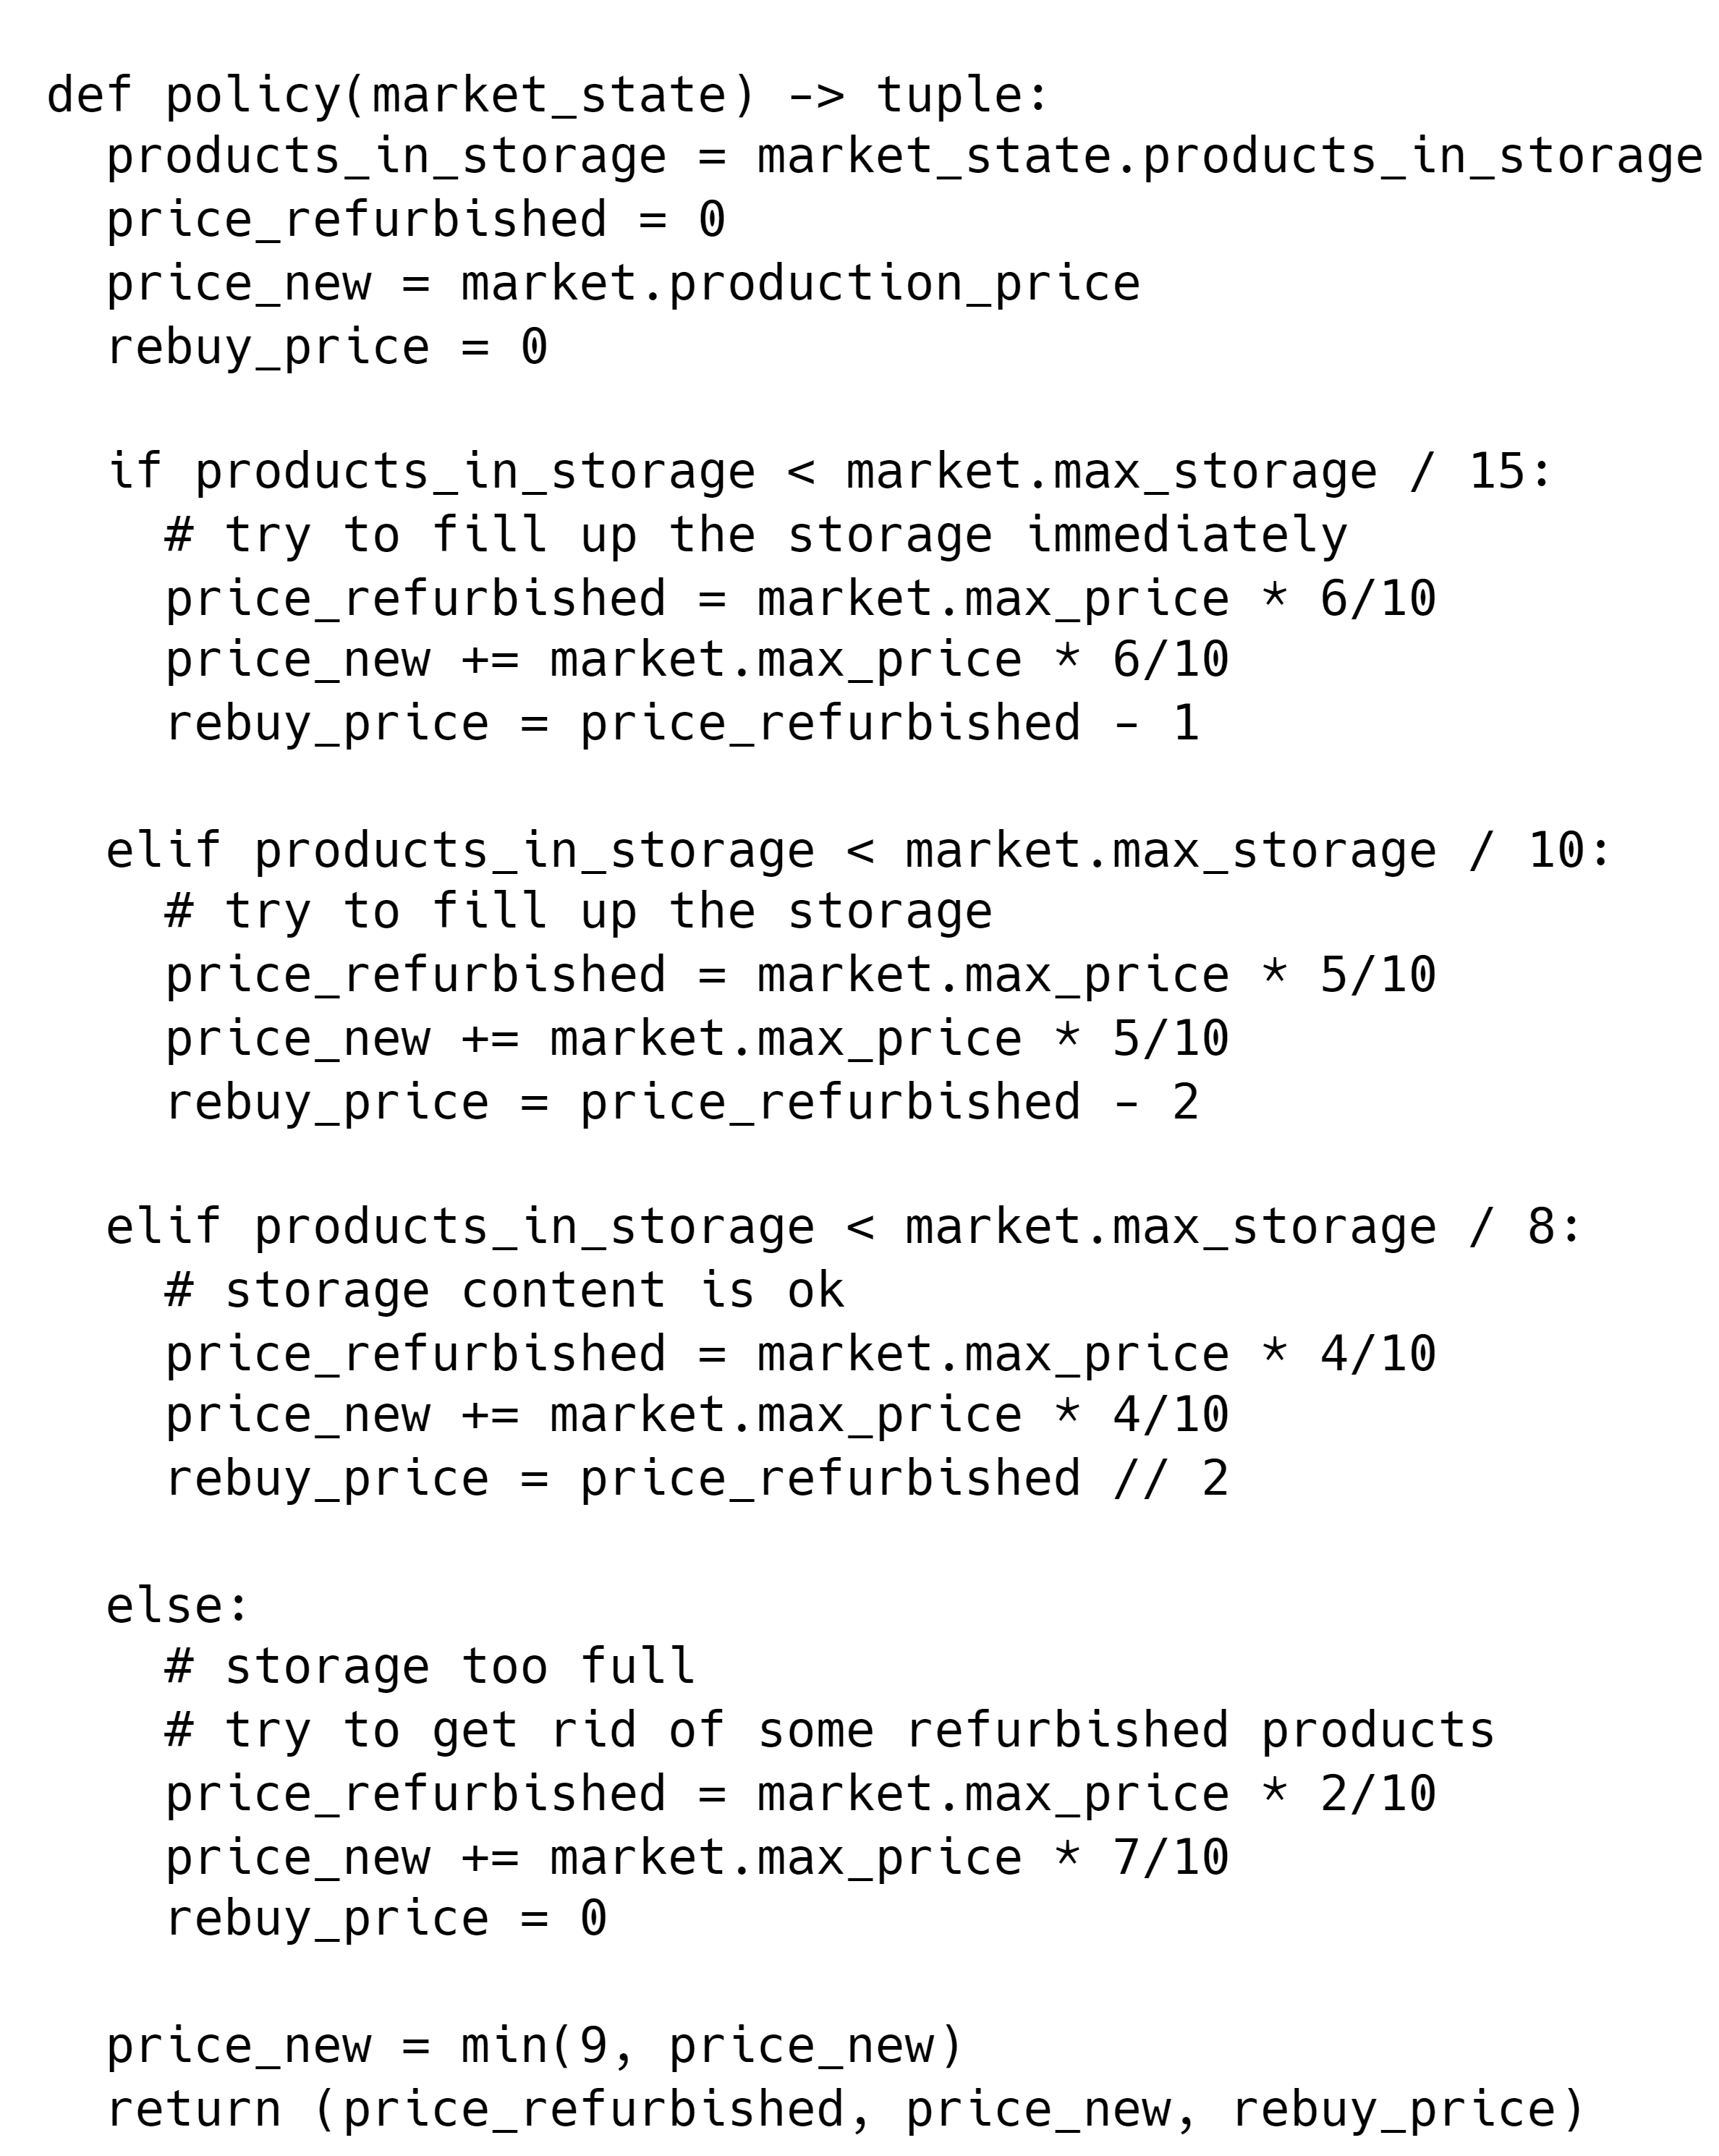
\includegraphics[width = \textwidth]{images/policies/RuleBasedCERebuyAgentPolicy.png}\\
	\caption{Policy implementation of the \emph{RuleBasedCERebuyAgent}, simplified for readability.}\label{fig:PolicyRuleBasedCERebuy}
\end{figure}

\begin{figure}[ht]
	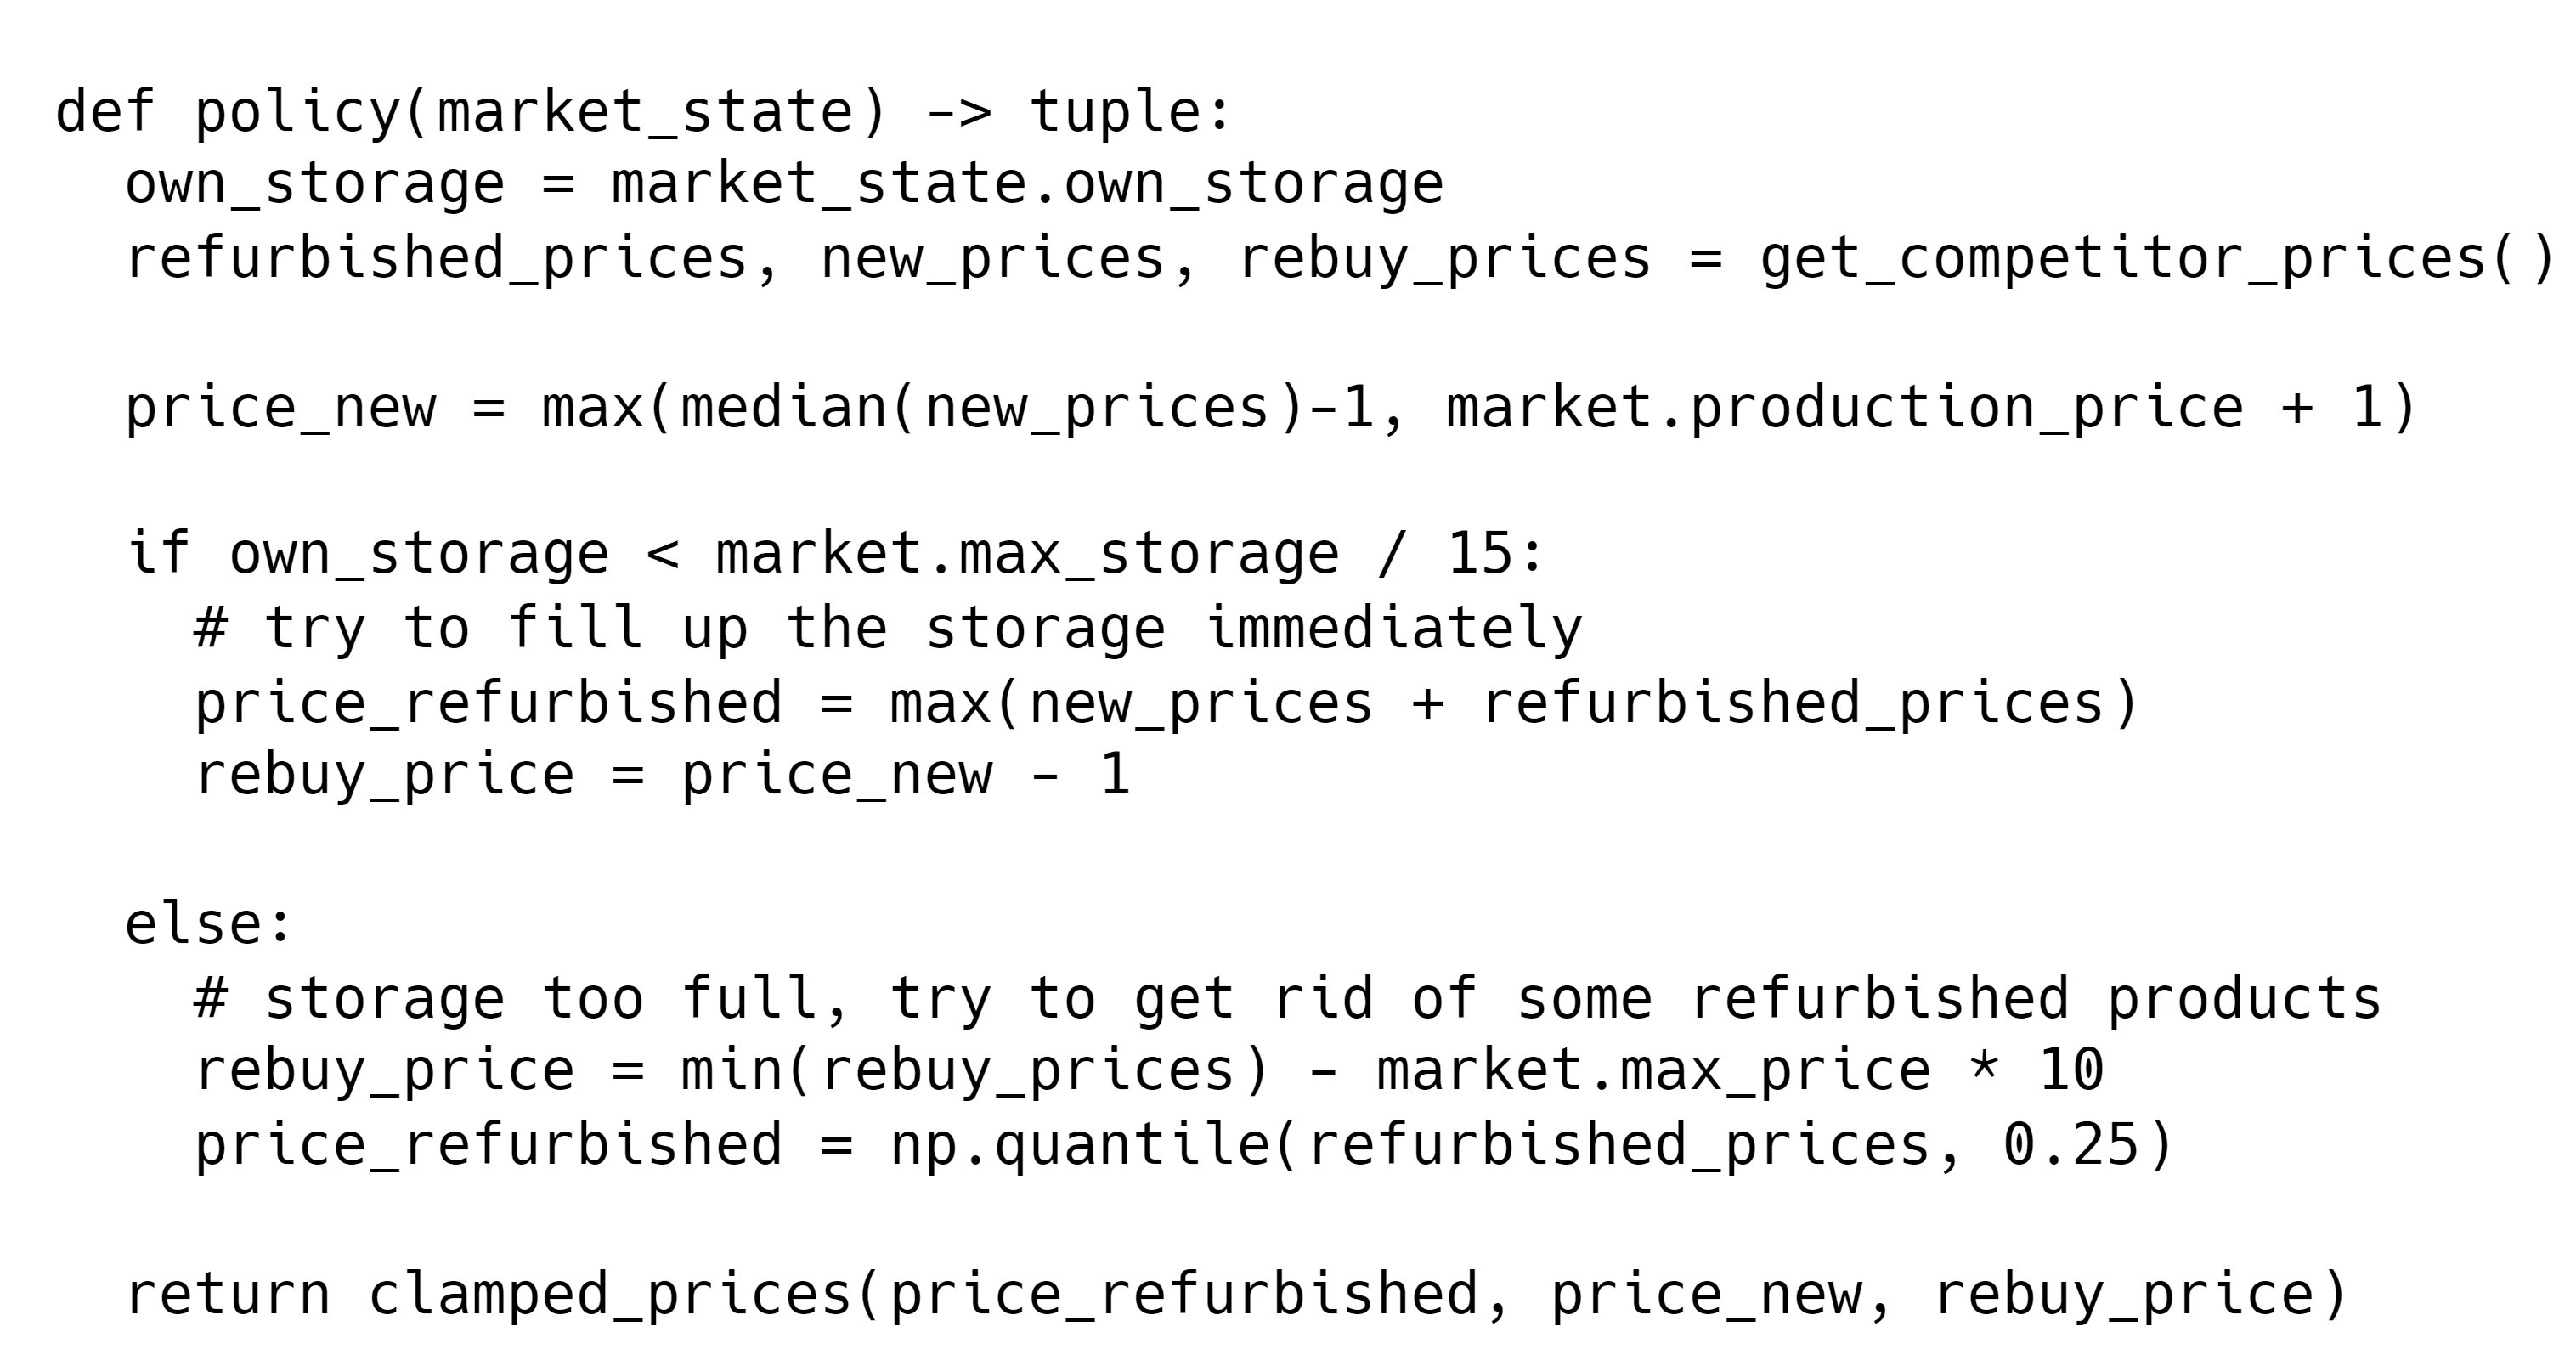
\includegraphics[width = \textwidth]{images/policies/RuleBasedCERebuyAgentStorageMinimizerPolicy.png}\\
	\caption{Policy implementation of the \emph{RuleBasedCERebuyAgentStorageMinimizer}, simplified for readability.}\label{fig:PolicyRuleBasedStorageMinimizer}
\end{figure}

\begin{figure}[!]
	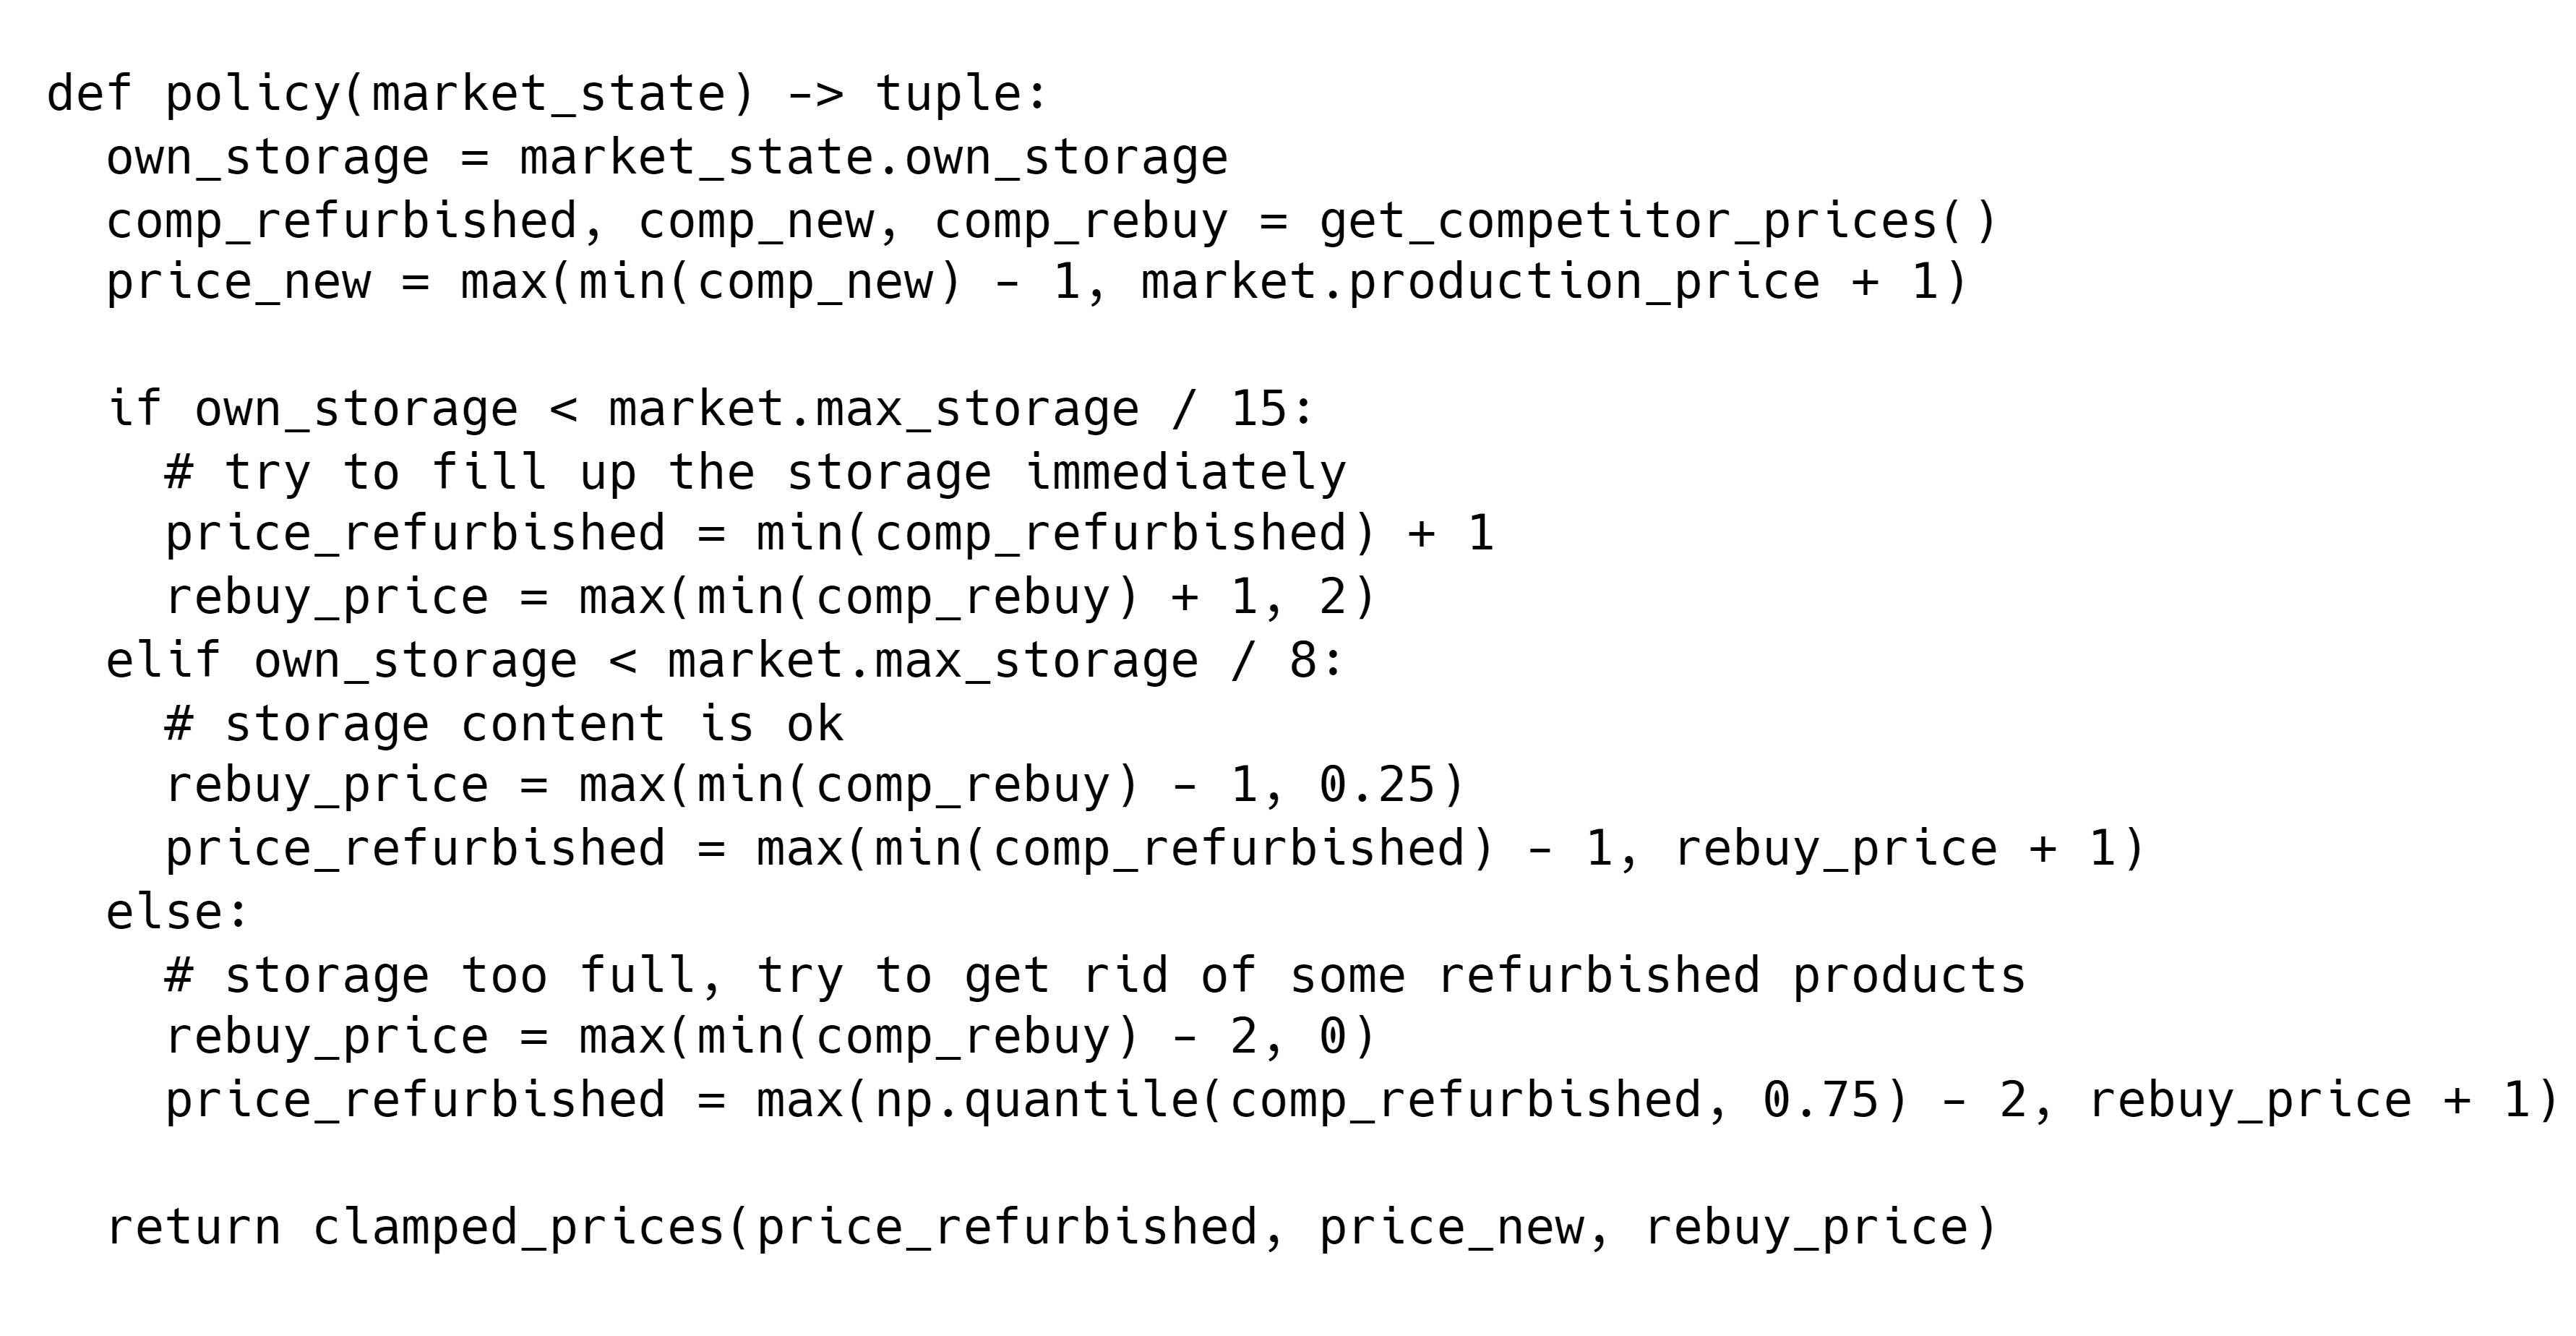
\includegraphics[width = \textwidth]{images/policies/RuleBasedCERebuyAgentCompetitivePolicy.png}\\
	\caption{Policy implementation of the \emph{RuleBasedCERebuyAgentCompetitive}, simplified for readability.}\label{fig:PolicyRuleBasedCompetitive}
\end{figure}

\clearpage
\section{SAC-Duopoly experiment - Configuration files}\label{sec:AppendixConfigFiles}

\begin{figure}[ht]
	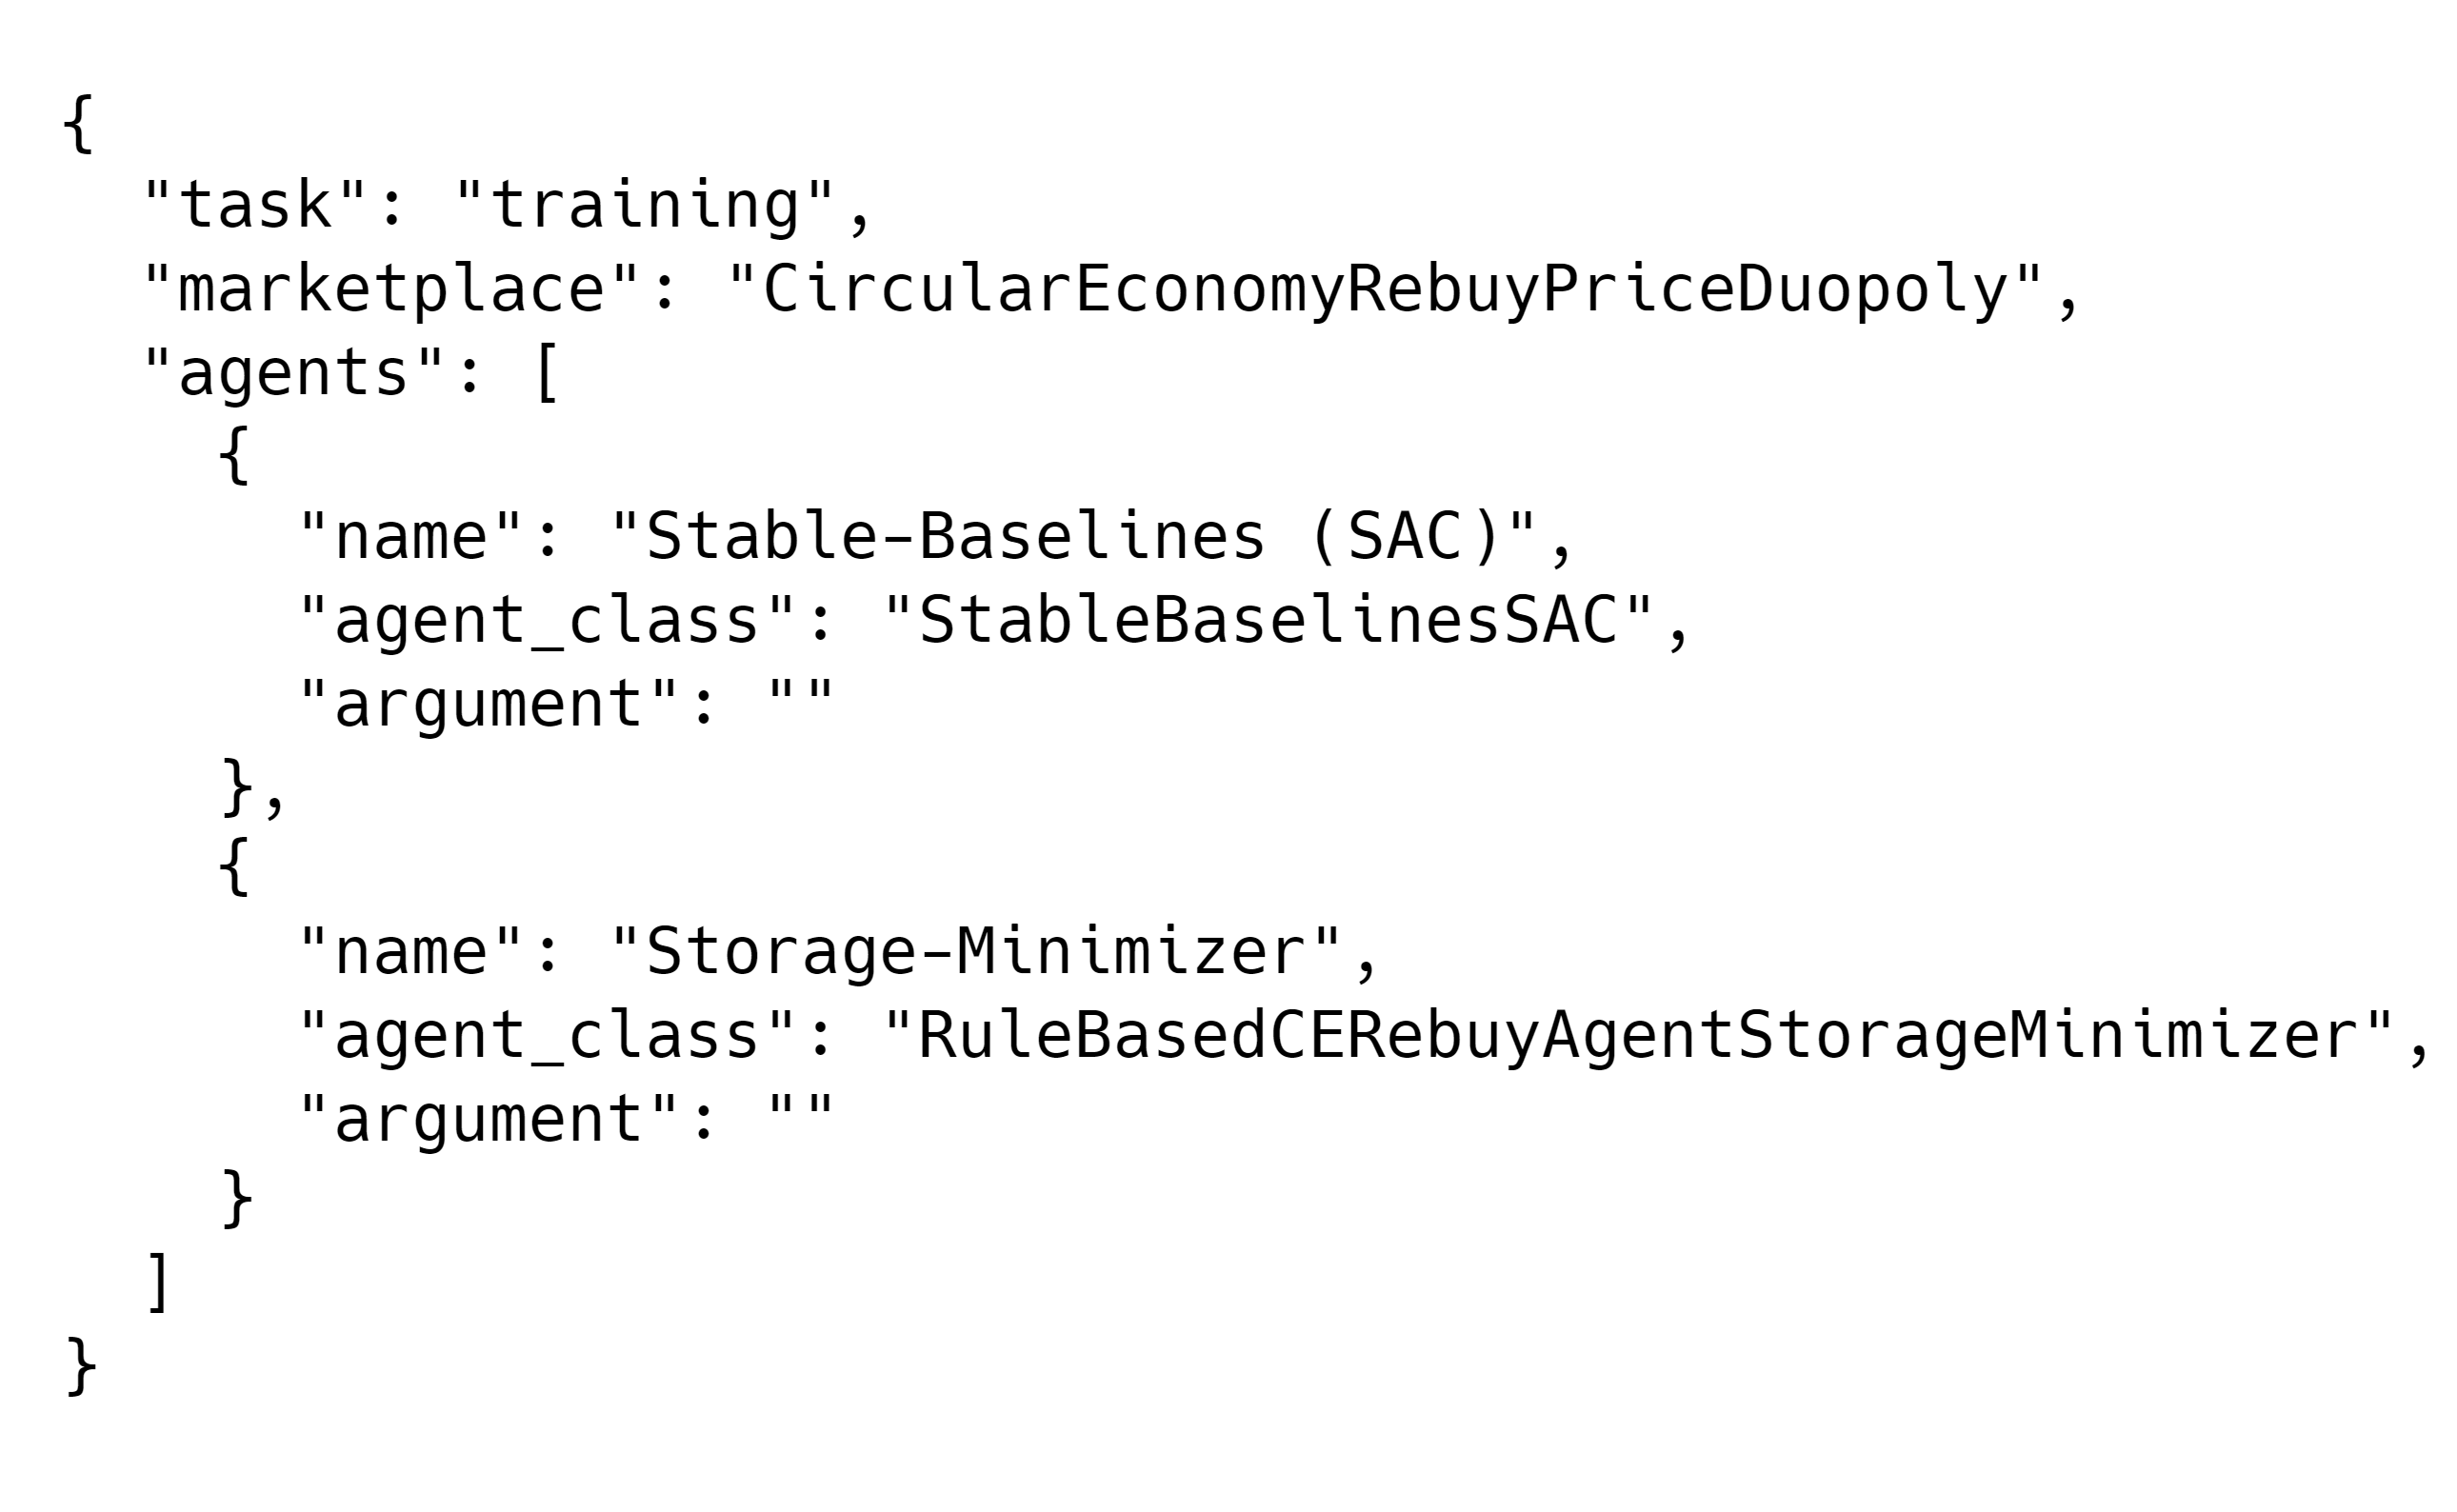
\includegraphics[width = \textwidth]{images/configs/SACDuopolyEnvironment.png}\\
	\caption{The \texttt{environment\_config.json} of the SAC-Duopoly experiment.}\label{fig:SACDuopolyConfigEnvironment}
\end{figure}

\begin{figure}[!]
	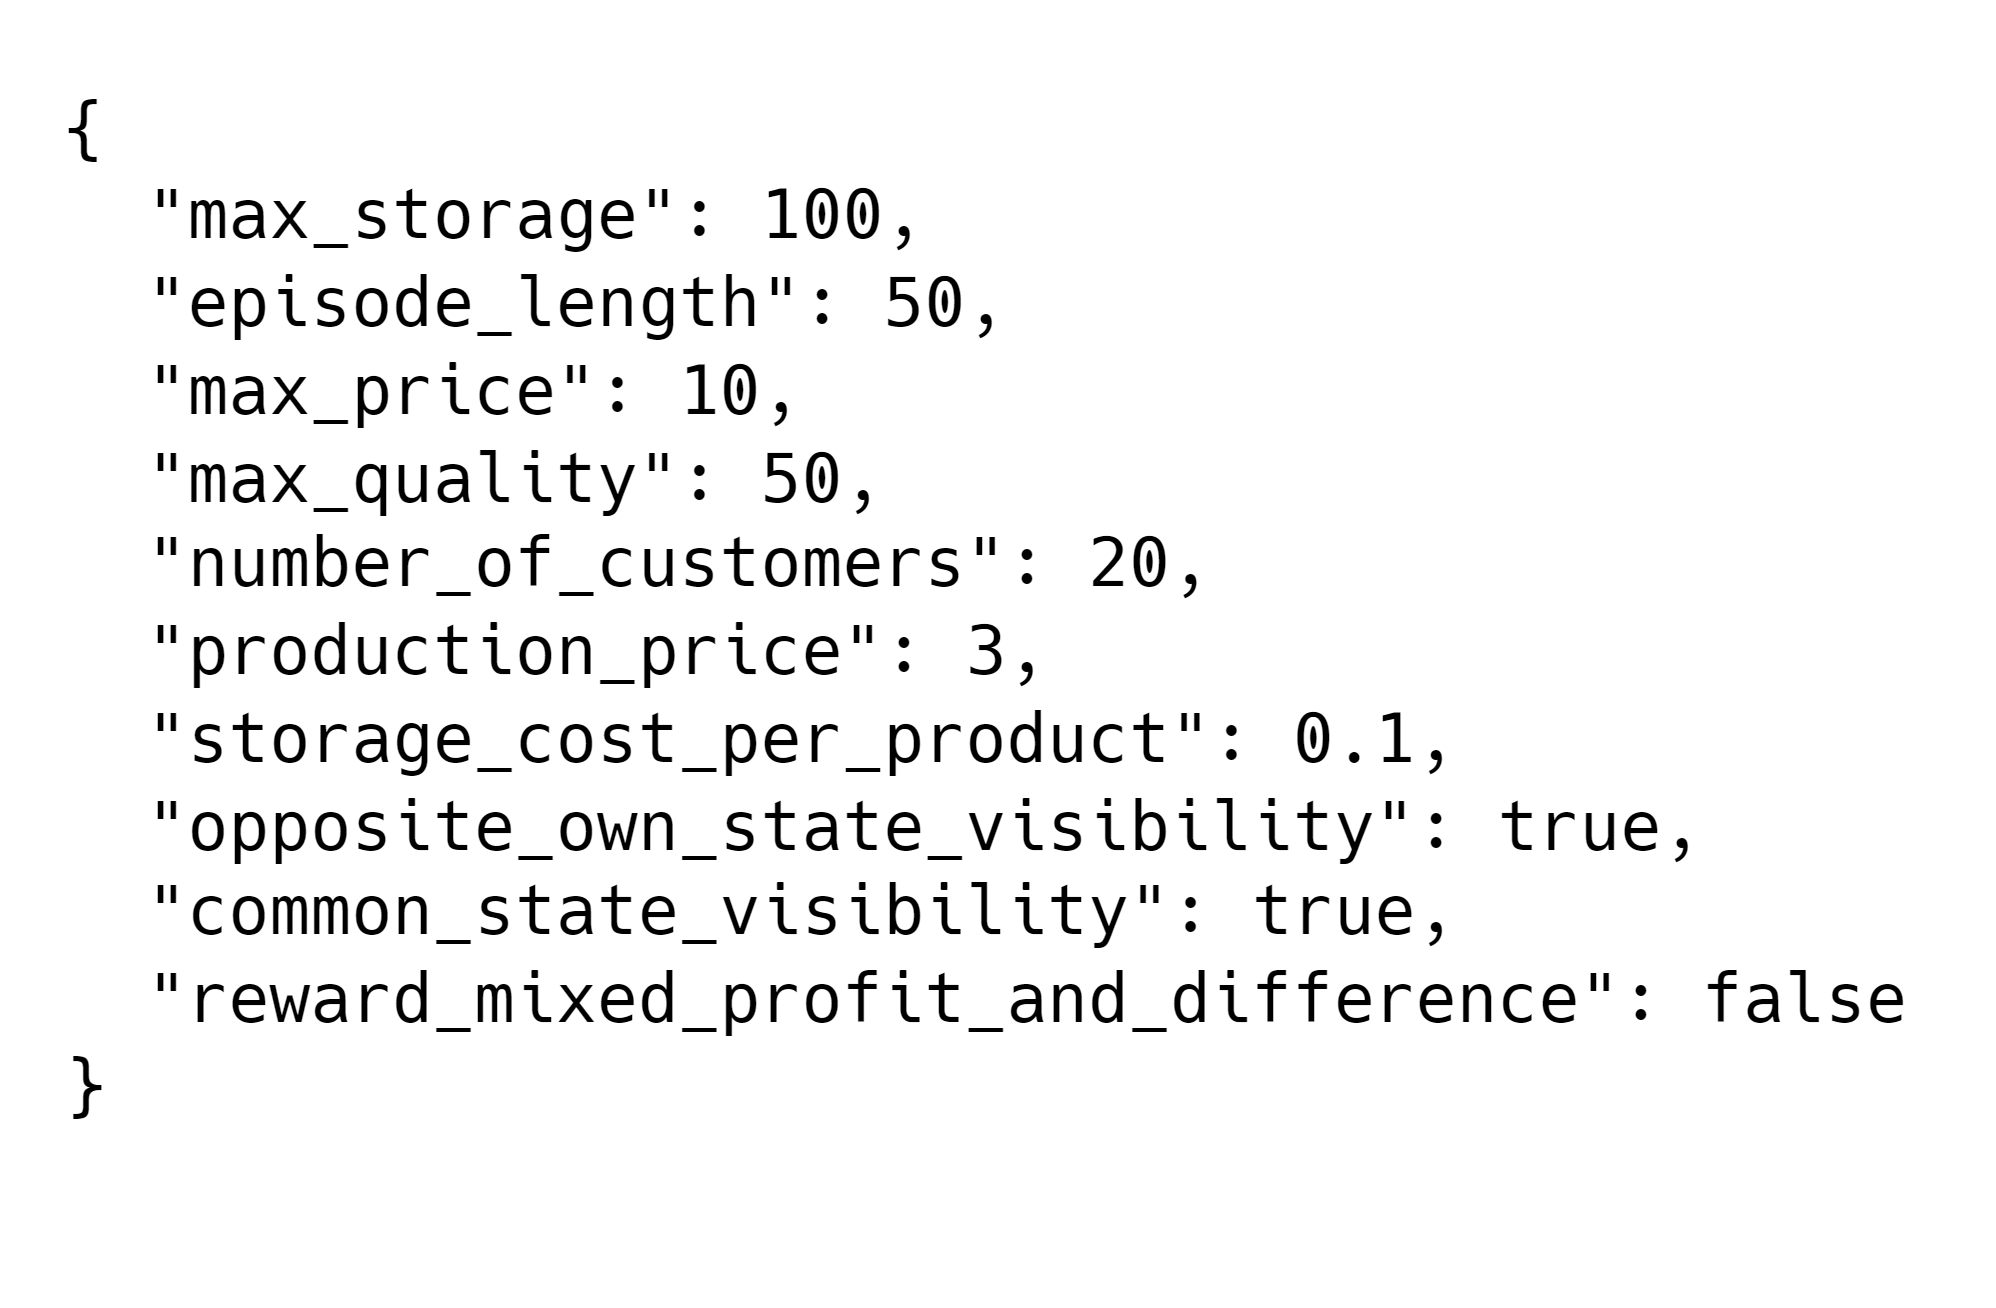
\includegraphics[width = 0.9\textwidth]{images/configs/SACDuopolyMarket.png}\\
	\caption{The \texttt{market\_config.json} of the SAC-Duopoly experiment.}\label{fig:SACDuopolyConfigMarket}
\end{figure}

\begin{figure}[ht]
	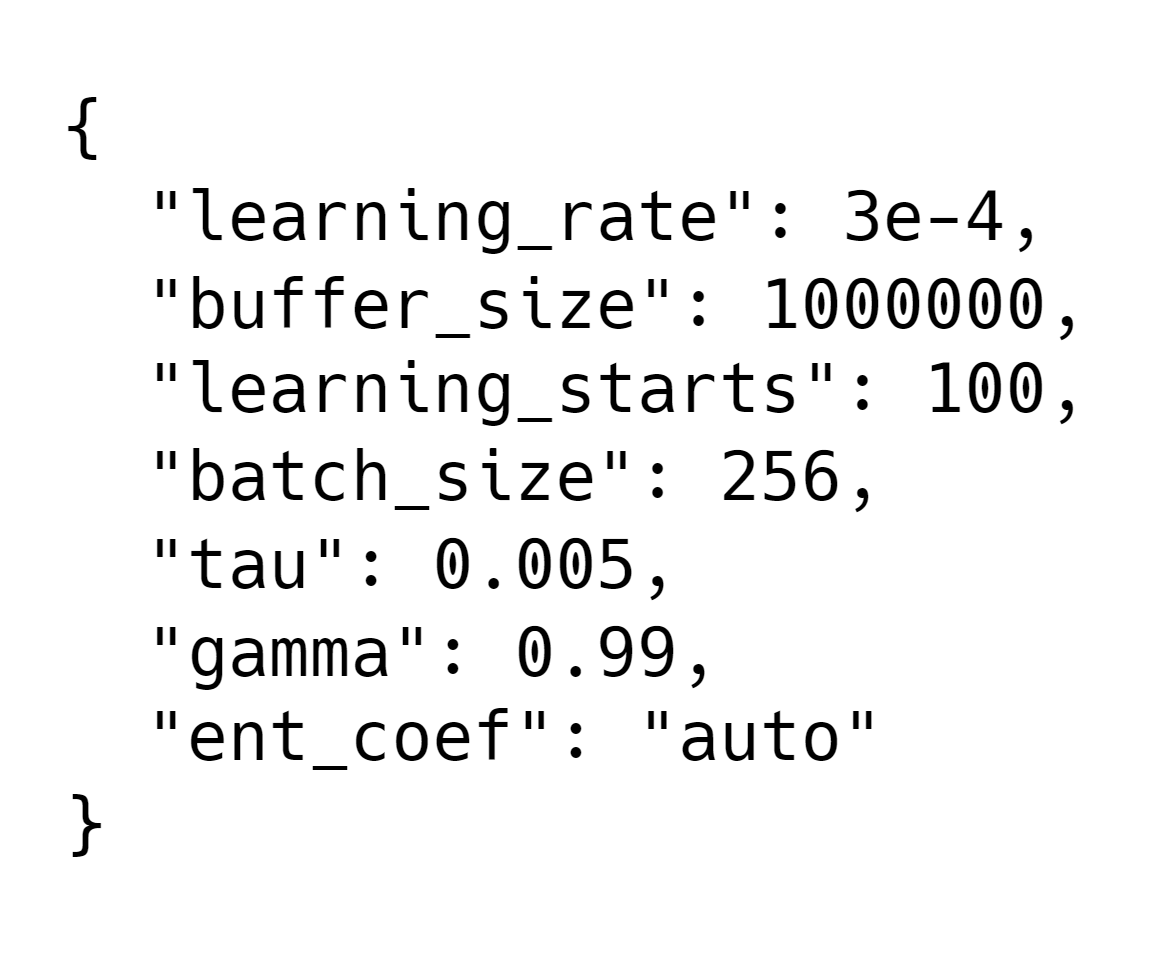
\includegraphics[width = 0.75\textwidth]{images/configs/SACDuopolyAgent.png}\\
	\caption{The configuration file for the SAC-Agent of the SAC-Duopoly experiment.}\label{fig:SACDuopolyConfigAgent}
\end{figure}

\clearpage
\section{PPO-Oligopoly experiment}\label{sec:AppendixOligopoly}

\subsection{Configuration files}\label{sec:AppendixOligopolyConfig}

\subsection{Diagrams}\label{sec:AppendixOligopolyDiagrams}

\begin{figure}[ht]
	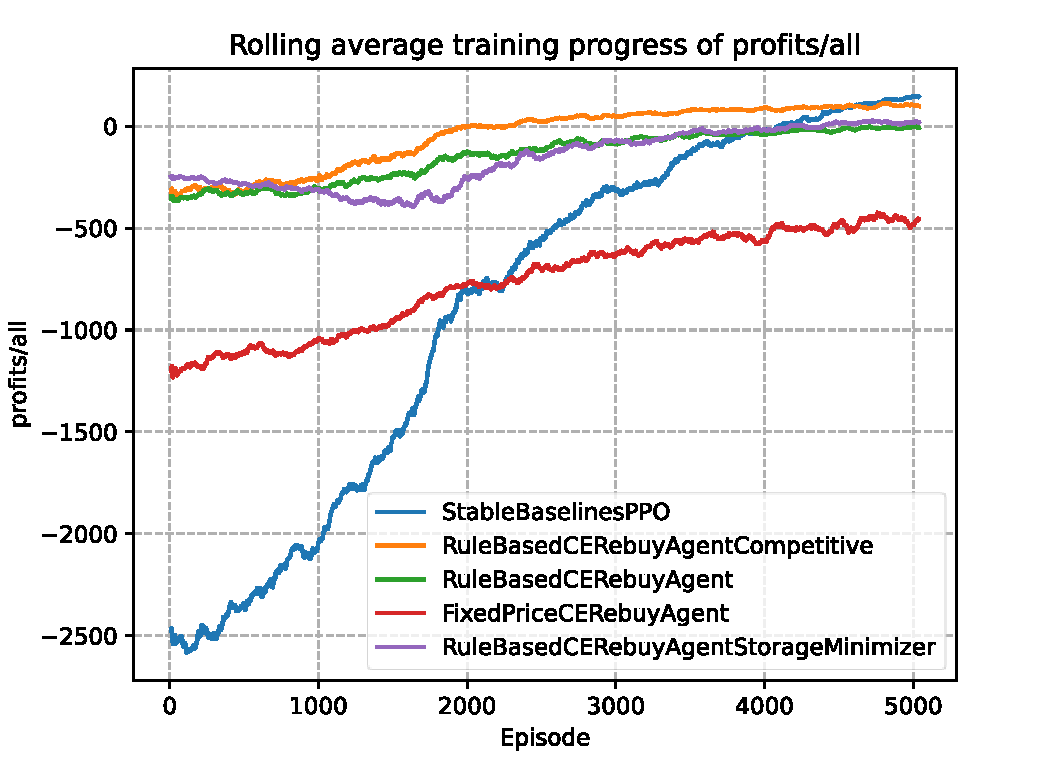
\includegraphics[width = 0.75\textwidth]{images/experiments/PPOOligopoly/LineProfitsAll.pdf}\\
	\caption{Mean profits achieved during the training run. The model was trained for 5,000 episodes.}\label{fig:PPOOligopolyLineProfitsAll}
\end{figure}